% 第6章第1节：顶点函数与边函数（顶点函数、边函数、沿边差分）。

\section{顶点函数与边函数}
\label{sec:graph-vertex-edge-functions}

谱方法处理的是挂在图上的数值。动手构造算子之前，先要说清三件事：数值放在哪里（顶点还是边），取什么值，允许做哪些运算。本节先分别建立顶点函数与边函数，再用关联矩阵实现从前者到后者的沿边差分。矩阵在这里只负责实现已经说明的作用，不代替对象本身的解释。

\subsection{顶点函数}
\label{sec:graph-spec-vertex-functions}

回到章首的传感器网络。每个测点给出一个温度读数，相当于给每个顶点指定一个实数，也就是一个映射$f:V\to\mathbb R$，称为\term{顶点函数}（vertex function），也常称为\term{图信号}（graph signal）。固定顶点的一个编号$V=\{1,\ldots,n\}$后，顶点函数可以存成向量$\bm f=(f_1,\ldots,f_n)^{\top}\in\mathbb R^n$，其中$f_i=f(i)$。全体顶点函数于是构成$n$维实向量空间：两个函数可以逐点相加、数乘，即$(\alpha\bm f+\beta\bm g)_i=\alpha f_i+\beta g_i$；也可以使用欧氏内积$\langle\bm f,\bm g\rangle=\sum_if_ig_i$和长度$\lVert\bm f\rVert_2$（第~\ref{sec:ls-inner-product-definition}节）。

编号只决定数值在数组中的位置，不改变数值属于哪个顶点。换一种编号，相当于用置换矩阵$\bm P$重排坐标，得到$\bm P\bm f$；第~\ref{sec:graph-isomorphism}节已经说明，邻接矩阵在重编号下同步变为$\bm P\bm A\bm P^{\top}$。本章后面的每个算子都要检查这一点：重编号后输出也只是随之重排，不能因为编号不同而改变结果。

并非所有挂在顶点上的数字都能这样运算。给顶点按类别标上$1,2,3$时，这些数字首先表示身份，“$1$号类与$3$号类的平均是$2$号类”没有意义，也不能把类别编号当温度求平均。处理类别标记的是第~\ref{sec:graph-wl-refinement}节的标记细化，它只比较相同与否和出现次数；本章只处理确实可以相加、数乘的数值。

一个测点有时同时记录温度、湿度等多个读数，可以把$c$个通道按列排成矩阵$\bm X\in\mathbb R^{n\times c}$。本章的节点算子都是$n\times n$矩阵，左乘$\bm X$时对每一列分别作用，各通道之间互不干扰；若要把不同通道混合，需要右乘一个$c\times c$矩阵，这是另一项操作，不属于图的结构。下文只讨论单个通道。

\subsection{边函数}
\label{sec:graph-spec-edge-functions}

数值也可以挂在边上：管道中的流量、两端读数之差、相邻两点间的作用量，都以边为索引。给每条边指定一个实数的映射$\varphi:E\to\mathbb R$称为\term{边函数}（edge function）；固定边的编号$e_1,\ldots,e_m$后，它存成$\bm\varphi\in\mathbb R^m$。与顶点函数一样，边函数也可以逐边相加、数乘，并带有欧氏内积。

无向边本身没有方向，但许多边上的数值带有符号。说“沿边$\{1,2\}$的流量是$3$”时，必须说明是从$1$流向$2$还是反过来；从$2$流向$1$的流量$3$，等于从$1$流向$2$的流量$-3$。因此记录有符号的边上数值之前，要给每条无向边选一个参考方向。这个方向只是记账约定：把某条边的参考方向反过来，对应的数值改变符号，所描述的物理量不变。这与有向图中弧的方向不同，后者属于图的结构，不能随意翻转。

无向边权是另一种情形。权$w_{i,j}=w_{j,i}\geq0$描述两端应当被比较的强度，不随方向改变符号，可以直接看成无向边上的函数。权与流量、差值的区别还在于计算中的角色：本章的算子把边权当作固定参数，把边差、流量这类量当作待处理的数值。以三点路径$1-2-3$为例，顶点函数是$\mathbb R^3$中的向量，边函数是$\mathbb R^2$中的向量；二者维数不同、索引不同，不能相加。

边权为零的结构边仍然属于边集$E$，第~\ref{chap:graph-traversal}、\ref{chap:graph-optimization}章的遍历与组合优化是否使用它，由那些问题自己的规则决定。本章的算子只受正权边影响，所以把它们单独收集起来：
\[
 E_+=\bigl\{\{i,j\}\in E:w_{i,j}>0\bigr\},
\]
称$(V,E_+)$为\term{正权支撑}图（positive-weight support graph），记$m_+=|E_+|$。按顶点编号把权排成对称矩阵$\bm W=[w_{i,j}]$，没有边的位置记$0$；按边编号把权排成对角矩阵$\bm W_E=\operatorname{diag}(w_{e_1},\ldots,w_{e_m})$。注意$\bm W$中的$0$不区分“无边”与“零权边”，需要区分时另存结构掩码（第~\ref{sec:graph-representations}节）。

\subsection{沿边差分}
\label{sec:graph-spec-edge-differences}

顶点函数最基本的沿边信息是每条边两端的差。第~\ref{sec:graph-representations}节的关联矩阵正好用来计算它：给每条无向边选定参考方向后，$\bm B\in\mathbb R^{n\times m}$的第$e$列在起点处为$1$、终点处为$-1$，其余为零。若边$e$从$i$指向$j$，则
\begin{equation}
 (\bm B^{\top}\bm f)_e=f_i-f_j .
 \label{eq:graph-spec-edge-difference}
\end{equation}
$\bm B^{\top}$把顶点函数映成边函数，记录每条边上“起点减终点”的差。由于$\bm B$的每一列恰有一个$1$和一个$-1$，常量函数$\bm1$的每条边差都为零：$\bm B^{\top}\bm1=\bm0$。

以三点路径为例，取参考方向$e_1:1\to2$、$e_2:2\to3$，顶点值$\bm f=(3,1,2)^{\top}$。此时
\[
 \bm B=\begin{bmatrix}1&0\\-1&1\\0&-1\end{bmatrix},\qquad
 \bm B^{\top}\bm f=\begin{bmatrix}3-1\\1-2\end{bmatrix}=\begin{bmatrix}2\\-1\end{bmatrix}.
\]
逐列核对：第一列表示$e_1$从$1$出发、到$2$结束，所以读出$f_1-f_2$；第二列读出$f_2-f_3$。

反方向的映射$\bm B$把边函数送回顶点：$(\bm B\bm\varphi)_i$等于以$i$为起点的边上数值之和减去以$i$为终点的边上数值之和，即按参考方向计算的净流出量。两个方向由转置联系，$\langle\bm B^{\top}\bm f,\bm\varphi\rangle=\langle\bm f,\bm B\bm\varphi\rangle$。下一节构造拉普拉斯时，先用$\bm B^{\top}$取边差，再用$\bm B$汇总回顶点。

\begin{figure}[!htb]
  \centering
  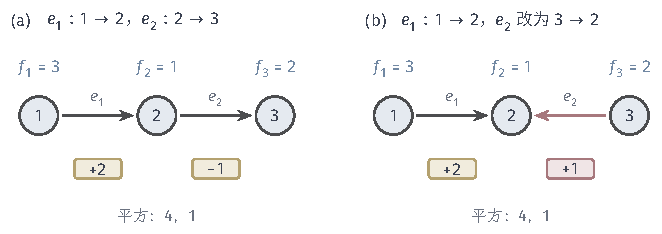
\includegraphics[width=112mm]{figures/01-basic-mathematics/04-graphs/tikz/c6-vertex-edge-functions/figure.pdf}
  \caption{三点路径上的顶点函数与边函数。蓝色数字是顶点值$\bm f=(3,1,2)^{\top}$，方框中是按参考方向计算的边差$(\bm B^{\top}\bm f)_e$（起点减终点）。(a)~$e_1:1\to2$、$e_2:2\to3$，边差为$(2,-1)$；(b)~只把$e_2$改记为$3\to2$（红色），它的边差变为$+1$。单条边差的符号随参考方向改变，平方$4$与$1$不变。}
  \label{fig:graph-spec-vertex-edge-functions}
\end{figure}

单条边差依赖参考方向。把$e_2$改记为$3\to2$，$\bm B$的第二列变号，该边的差从$f_2-f_3=-1$变成$f_3-f_2=1$，而$e_1$的差不受影响，见图~\ref{fig:graph-spec-vertex-edge-functions}。用矩阵表示，一次改记相当于右乘一个对角元为$\pm1$的符号矩阵$\bm R$（改记的边取$-1$），新关联矩阵为$\bm B\bm R$，新边差为$\bm R\bm B^{\top}\bm f$：每个分量至多变号，绝对值与平方都不变。由此得到构造无向图算子的一条要求：结果只能依赖边差的平方或其他不受符号影响的组合，否则它描述的是记账方式，而不是图本身。下一节的拉普拉斯满足这一要求。
